\documentclass{article}
\usepackage[T1]{fontenc}
\usepackage{lmodern}
\usepackage{graphicx}
\usepackage{amsmath,amssymb}
\usepackage[a4paper,margin=2cm]{geometry}
\usepackage[absolute,overlay]{textpos}
\setlength{\TPHorizModule}{1mm}
\setlength{\TPVertModule}{1mm}
\usepackage[indonesian]{babel}
\usepackage{hyperref}
\setlength{\emergencystretch}{2em}
% unit: Halaman 92

\begin{document}

% === Halaman 92 (python/native) ===

3. Column round dan diagonal round

92

// Column round

QR(0, 4,  8, 12)         // kolom 1

QR(1, 5,  9, 13)         // kolom 2

QR(2, 6, 10, 14)       // kolom 3

QR(3, 7, 11, 15)       // kolom 4

// Diagonal round

QR(0, 5, 10, 15) 

// diagonal 1 

QR(1, 6, 11, 12) 

// diagonal 2

QR(2, 7,  8, 13)             // diagonal 3

QR(3, 4,  9, 14) 

// diagonal 4

% deskripsi: gambar native xref 321
\noindent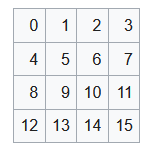
\includegraphics[width=0.85\textwidth]{../../images/python/page_092_img_01.png}

\end{document}
